\documentclass[a4paper]{article}
\usepackage[a4paper,top=2.5cm,bottom=2.5cm,left=3cm,right=3cm,% margins
    headheight=1.5cm,headsep=1.5em,
    footskip=2em,
]{geometry}

% 载入常用的数学包, 符号包
\usepackage{amsmath}
\usepackage{amsfonts}
\usepackage{amssymb}
\usepackage{mathrsfs}
\usepackage{blindtext}

%% linespace 行间距,段间距等等
\usepackage{setspace}
% \usepackage{indentfirst} % then the first line of each title should start with a indent.
% 定义标题和段落样式
% 定义1.5倍行距
\renewcommand{\baselinestretch}{1.62}
\setlength{\baselineskip}{12pt}   % set the fixed value of the lineskip
\setlength\parskip{\baselineskip} % set the space between the paragraphs, set the variable \parskip \baselineskip
% parindent
\setlength{\parindent}{0pt}

% fonts (style, color, size). 
\usepackage{ctex}		 	% If you are lazy, the CTEX suit is enough.

% Chinese font
\usepackage{xeCJK}		 	% For the Chinese through XeLaTex
\setCJKmainfont{FandolSong} 	% set the mainfont of Chinese as songti. (serif) for  
\setCJKsansfont{FandolSong}	% sans serif font for \textsf
\setCJKmonofont{FandolSong}	% monospace font for \texttt
% \punctstyle{kaiming}   	% Remove the space used by symbols like comma. Special for the mainland students like us HUSTers.
\setCJKfamilyfont{song}{FandolSong}
\newcommand{\song}{\CJKfamily{song}} %宋体 song
\setCJKfamilyfont{kai}{FandolKai}
\newcommand{\kai}{\CJKfamily{kai}} %楷体2312  kai
\setCJKfamilyfont{hwzs}{FandolFang}
\newcommand{\hwzs}{\CJKfamily{hwzs}} %华文中宋  hwzs
\setCJKfamilyfont{hei}{FandolHei}
\newcommand{\hei}{\CJKfamily{hei}} %黑体  hei

% English font
\usepackage{fontspec}
\setmainfont{Times New Roman}
\setsansfont{Times New Roman}
\setmonofont{Times New Roman}
% font Color 利用definecolor自己可以定义颜色
\usepackage{xcolor}
\definecolor{MSBlue}{rgb}{.204,.353,.541}
\definecolor{MSLightBlue}{rgb}{.31,.506,.741}
% font Size 
\newcommand{\xiaochuhao}{\fontsize{36pt}{\baselineskip}\selectfont}
\newcommand{\erhao}{\fontsize{21pt}{\baselineskip}\selectfont}
\newcommand{\xiaoerhao}{\fontsize{18pt}{\baselineskip}\selectfont}
\newcommand{\sanhao}{\fontsize{15.75pt}{\baselineskip}\selectfont}
\newcommand{\sihao}{\fontsize{14pt}{18pt}\selectfont}
\newcommand{\xiaosihao}{\fontsize{12pt}{18pt}\selectfont}
\newcommand{\wuhao}{\fontsize{10.5pt}{18pt}\selectfont}

%% header and footer 
\usepackage{fancyhdr} % for header and footer
% header
\newcommand{\headstyle}{
    \fancyhead[L]{ \hwzs\wuhao 《面向对象程序设计语言》课程设计报告}
    \fancyhead[R]{ \hwzs\wuhao 162210118~魏程浩}
}
% 设置页脚样式
\newcommand{\footstyle}{\fancyfoot[C]{\wuhao\thepage}
    \fancyfoot[L]{\rule[5pt]{6.7cm}{0.4pt}}
    \fancyfoot[R]{\rule[5pt]{6.7cm}{0.4pt}}
}
\pagestyle{fancy}
\fancyhf{} % 清空原有样式
\headstyle
\footstyle
% 定义一种新的格式叫做main
\fancypagestyle{main}{%
    \fancyhf{} % 清空原有样式
    \headstyle
    \footstyle
}
\renewcommand{\headrulewidth}{0.4pt}
% \renewcommand{\footrulewidth}{0.4pt}
% \renewcommand{\headrule}{\rule{\textwidth}{0.4pt}}

% set the styles of sections at all levels
\usepackage{titlesec}
\usepackage{titletoc}
\titleformat{\section}{\centering\hei\bfseries\xiaoerhao}{\thesection}{1em}{} % 在section标题编号后面加个点
\titleformat*{\subsection}{\raggedright\hei\bfseries\sihao}
\titleformat*{\subsubsection}{\raggedright\hei\bfseries\xiaosihao}
\titleformat{\paragraph}[hang]{\raggedright\hei\bfseries\xiaosihao}{\theparagraph}{1em}{}[]

% manual
% \titleformat{command}[shape]{format}{label}{sep}{before-code}[after-code]
% \titlespacing{command}{left}{before-sep}{after-sep}
% 设置新的层级subsubsubsection
\setcounter{tocdepth}{4}
\setcounter{secnumdepth}{4}

\newcommand{\sectionbreak}{\clearpage} % 小节从新的一页开始
% 根据学校要求设置新的section, subsection, subsection,  paragraph

% set the content of section and so on
\newcommand\seccontent{
    \song
    \xiaosihao % 默认五号字体, 行间距为1.5*\baselineskip
    \setlength{\parindent}{2em} % 首段缩进两个M字符
    \setlength{\parskip}{0pt}
}
\newcommand\tabcontent{
    \song
    \wuhao % 默认五号字体, 行间距为1.5*\baselineskip
    \setlength{\parindent}{2em} % 首段缩进两个M字符
    \setlength{\parskip}{0pt}
}

% ---------------------------------------------------------------------------- %
% for the style of theorems, definitions, proofs and remarks 定义数学里面一些常用的环境
\usepackage{amsthm}
\newtheorem{thm}{\textbf{定理}}[section]
% The section in [] can be replaced by chapter or subsection
\theoremstyle{definition}
\theoremstyle{plain}
\theoremstyle{remark}

% ---------------------------------------------------------------------------- %
% for the caption and reference 图表及公式的编号规范
\usepackage{float} 		 		  	% table figure positioning
\usepackage{caption}
\captionsetup[figure]{labelformat=default, labelsep=quad,name={图}}
\captionsetup[table]{labelformat=default,labelsep=quad,name={表}}
% 设置图表标题的计数方式
\renewcommand{\thefigure}{\ifnum \thesection>0 \thesection-\fi \arabic{figure}} % set caption label style to 2-1
\renewcommand{\thetable}{\ifnum \thesection>0 \thesection-\fi \arabic{table}} % set caption label style to 2-1
\DeclareCaptionFont{mylabelfont}{\hei\xiaosihao}
\captionsetup[figure]{font=mylabelfont}
\captionsetup[table]{font=mylabelfont}

% 设置图表的autoref的格式
\newcommand{\reffig}[1]{图 \ref{#1}}
\newcommand{\reftab}[1]{表 \ref{#1}}
% 公式的编号格式
\renewcommand\theequation{\arabic{section}-\arabic{equation}}

\usepackage{graphicx} % To include graphixs 添加图所需的包
\usepackage{booktabs} % To create three line table including the commands toprule, bottomrule, and midrule
% 使用tabularx库并定义新的左右中格式
\usepackage{tabularx}
\usepackage{makecell}
\newcolumntype{L}{X}
\newcolumntype{C}{>{\centering \arraybackslash}X}
\newcolumntype{R}{>{\raggedright \arraybackslash}X}

% ---------------------------------------------------------------------------- %
% set the style of counters
\makeatletter
\@addtoreset{footnote}{page}
\@addtoreset{figure}{section}
\@addtoreset{table}{section}
\@addtoreset{equation}{section}
\makeatother

% ---------------------------------------------------------------------------- %
% tableofcontents, listoftables and listoffigures 目录
%\renewcommand\listfigurename{插图列表}
%\renewcommand\listtablename{表格列表}
%\titlecontents{标题名}[左间距]{标题格式}{标题标志}{无序号标题}{指引线与页码}[下间距]
%\dottedcontents{section}[2.55em]{\song \xiaosihao \bfseries}{2.5em}{1em}
\usepackage{tocloft}
\renewcommand{\contentsname}{\centerline{ \hei\bfseries\xiaoerhao 目\hspace{2em}录}}
\titlecontents{section}[3em]{\song\xiaosihao\bfseries}{\contentslabel{3em}}{\hspace*{-3em}}{\normalfont\titlerule*[8pt]{.}\contentspage}
\titlecontents{subsection}[3em]{\song\xiaosihao}{\contentslabel{3em}}{\hspace*{-3em}}{\titlerule*[8pt]{.}\contentspage}
\titlecontents{subsubsection}[4em]{\song\xiaosihao}{\contentslabel{4em}}{\hspace*{-4em}}{\titlerule*[8pt]{.}\contentspage}
\titlecontents{paragraph}[5em]{\song\xiaosihao}{\contentslabel{5em}}{\hspace*{-5em}}{\titlerule*[8pt]{.}\contentspage}

% reference and citation 参考文献
\usepackage{natbib}
\renewcommand{\refname}{\centering\hei\xiaoerhao 参考文献}
\bibsep=0pt % 用来设置每个\bibitem之间的间距
% \newcommand{\upcite}[1]{\textsuperscript{\textsuperscript{\cite{#1}}}} % show citation label in the upperscript

% 使用特殊符号
\usepackage{amssymb}
\usepackage{wasysym}

% 制作tatement中的符号
\def\HUSTcheckedbox{$\Square\!\!\!\!\checkmark$}
\def\HUSTbox{$\Square$}

\newcommand{\makestatement}[2]{\statement{#1}{#2}}

\usepackage{enumitem}
\setlist{noitemsep}

\usepackage{listings} % For the code. 代码
\usepackage[bookmarks=true,colorlinks,linkcolor=black,citecolor=black,urlcolor=purple]{hyperref}
\usepackage{appendix}
\renewcommand{\appendixname}{附录}

% titlepage
\usepackage{titling}
% 重置命令 maketitle
\renewcommand{\maketitle}{
    \def\HUSTtitlelength{12em}
    \begin{titlepage}
        \begin{center}
            \vspace*{0em}
            
\includegraphics[height=1.61cm]{fig/name.png}\\
            \vspace*{4em}
            {\xiaochuhao \hwzs \bfseries 《面向对象程序设计语言》课程设计报告}\\
            \vspace*{6em}
            {\erhao \kai \bfseries \thetitle}

            \vspace*{6em}
            {\sanhao \hwzs
                \renewcommand\arraystretch{2}
                \begin{tabular}{lc}
                    % \makebox[4em][s]{院 \hfill 系} &
                    % \underline{\makebox[\HUSTtitlelength]{\school}} \\
                    \makebox[4em][s]{专业}         &
                    \underline{\makebox[\HUSTtitlelength]{\major}}     \\
                    \makebox[4em][s]{班级}         &
                    \underline{\makebox[\HUSTtitlelength]{\class}}     \\
                    \makebox[4em][s]{姓 \hfill 名} &
                    \underline{\makebox[\HUSTtitlelength]{\theauthor}} \\
                    \makebox[4em][s]{学 \hfill 号} &
                    \underline{\makebox[\HUSTtitlelength]{\studentId}} \\
                    % \makebox[4em][s]{指导教师} &
                    % \underline{\makebox[\HUSTtitlelength]{\instructor}} \\
                    % 	\makebox[4em][s]{日\hfill 期} &
                    % \underline{\makebox[\HUSTtitlelength]{\thedate}} \\
                \end{tabular}
            }

            \vspace{4em}
            {\sanhao \hwzs \thedate}
        \end{center}
    \end{titlepage}
}

\newcommand{\hongzifuzhu}[1]{\textcolor{red}{\kai \wuhao(#1)}}

\title{title}
\def\major{major}
\def\class{classid}
\author{name}
\def\studentId{id}

\date{\today}

\begin{document}

\maketitle
\begin{spacing}{1.2}%魔法参数,行间距
    \tableofcontents
\end{spacing}
\thispagestyle{main}

\clearpage
\setcounter{page}{1}
\renewcommand{\thepage}{\arabic{page}}
\section{使用说明}\seccontent
\begin{description}
	\seccontent
    \item[模版来源] 
    本课程设计模版在华中科技大学本科毕业论文(设计)的基础上修改而来。
	\item[源模版信息] 
    作者:L0v3ch4n \href{https://github.com/Cuber-Wei}{@L0v3ch4n}。
    模板文本来源:冯洲 \href{https://github.com/zfengg}{@zfengg}。
    版本信息:2025/08/20 v1.0.0。
	\item[本地编译条件]  
    安装最新版本的 \href{http://www.tug.org/texlißve/}{TeXLive}(推荐)或 \href{http://miktex.org/}{MiKTeX}。
    请确保所有宏包都更新至最新。因为中文支持利用的是包\textbf{XeCJK},所以编译器请使用 Xe\LaTeX。 
    编辑器推荐 \href{http://texstudio.sourceforge.net/}{TeXstudio} 和 \href{https://code.visualstudio.com/}{Visual Studio Code}。 
    源模版在 Windows, Linux, MacOS 编译通过。更改后未测试。
	\item[图表引用] 图标的编号及题注已设计符合要求,如要引用, 请使用$\backslash$reffig$\lbrace\rbrace$ 引用图,$\backslash$reftab$\lbrace\rbrace$引用表格,以达到要求样式。
	\item[公式交叉引用] 方程的编号已调好,但是引用的格式没有另外设计,引用请使用自带的$\backslash$ref$\lbrace\rbrace$。
	\item[参考文献] 将bibtex粘贴到.bib文件中进行引用。bibtex文件的获取可在\href{https://scholar.google.com}{Google Scholar}网页中查找论文后点击下方的cite按钮,在pop page中点击bibtex。
    \item[LaTeX公式转换] 图片转LaTeX公式工具推荐\href{https://snip.mathpix.com}{@snip}需注册,免费版有每月100张图片的限制。

\end{description}

\section{项目描述}
\subsection{项目背景}
\subsubsection{室内定位}
\textit{随着智能设备的普及},基于位置的服务(LBS)成为人们日常生活中必不可 少的一部分。现代人有 80\%的时间是在室内度过的。如何在室内环境中准确地确 定用户的位置,
成为近年来的一个热门研究课题。

在室外空间,以 GPS、北斗为代表的卫星定位系统能够满足人们在户外开阔 环境中的定位需求;但在室内环境中,由于建筑结构、室内障碍物对卫星信号的 阻挡和反射,卫星定位系统会产生较大的定位误差。

因此,研究者们提出了多种基于无线信号的室内定位方案,利用的信号包括 Wi-Fi、蓝牙、超声波、超宽带、惯性传感器、红外线、声信号等。

\subsubsection{行人航位推算}
在行人定位领域\cite{qbz},行人航位推算(PDR\cite{li2019rmaptafa})是一种主流方法。传统的PDR算法依赖惯性测量单元(Inertia Measurement Unit,IMU)
收集行人的加速度、角速度等信息,进而推算行人的运动轨迹,见\reffig{pdrfig}。

\begin{figure}[htbp]
	\centering
	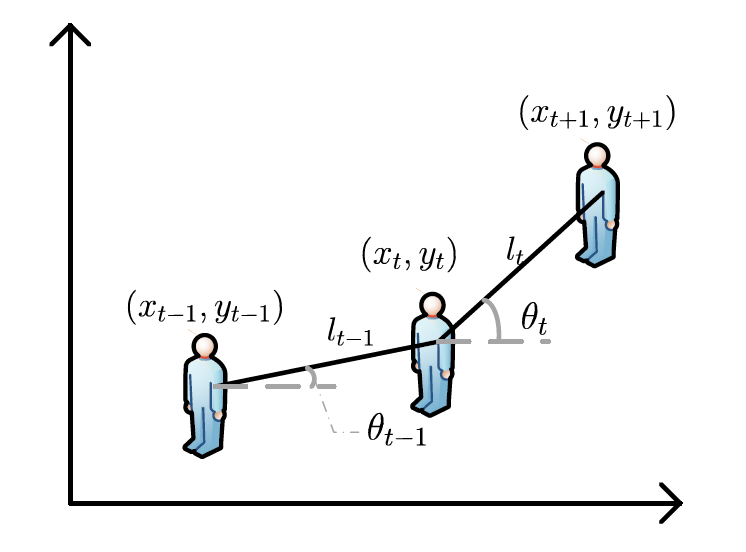
\includegraphics[width=0.5\textwidth]{fig/pdr.png}
	\caption{PDR示意图}
	\label{pdrfig}
\end{figure}

$$ x_t = x_{t-1} + l_{t-1} \times \cos \theta_{t-1} $$
$$ y_t = y_{t-1} + l_{t-1} \times \sin \theta_{t-1} $$

假设前一步点的位置为$(x_{t-1},y_{t-1})$,$t-1$到$t$时刻之间的步长为$l_{t-1}$,行进
方向角度为$\theta_{t-1}$。根据上式即可解出$t$时刻行人的估计位置$(x_t, y_t)$。

PDR算法主要包括步频检测、步长估计、航向估计三个任务。
\subsubsection{基础PDR算法}
\begin{itemize}
    \item 步频检测:波峰测频法 
    
    被测人员走动且手持终端时,随着人的周期性运动,三轴加速度传感器的波形也会产生周期性的变化,见\reffig{accxyz},其中以竖直方向(Z轴)上的加速度变化最为明显。当一个有效波峰出现,即可认为移动了一步。按此原理即可估计出行人的步频。
    \begin{figure}[htbp]
    	\centering
    	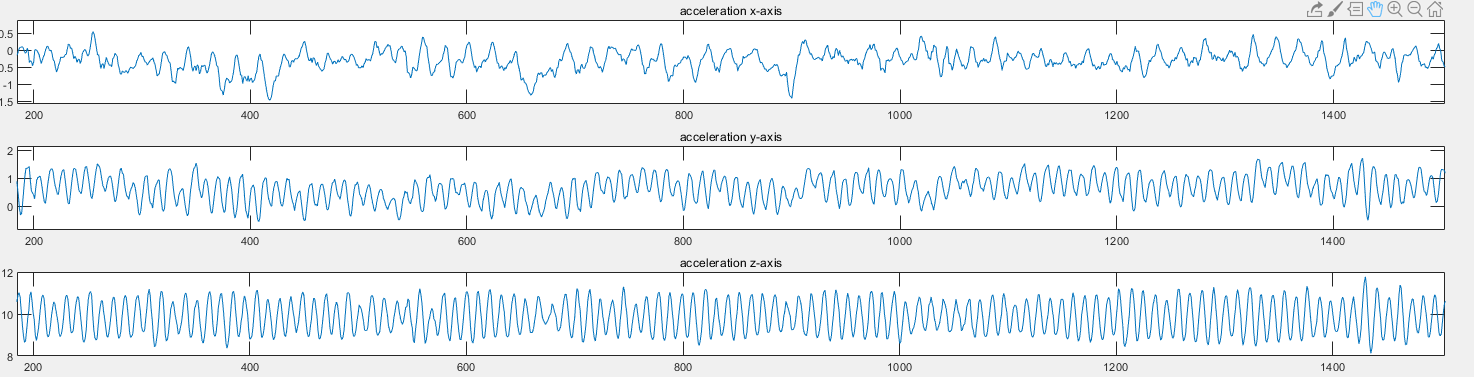
\includegraphics[width=0.75\textwidth]{fig/accxyz.png}
    	\caption{三轴加速度传感器的波形}
    	\label{accxyz}
    \end{figure}  
    \item 步长估计:Weinberg算法 
    
    步长估计利用Weinberg算法实现,与最大加速度和最小加速度相关。
    $$ l_n = K \times \left( a_n^{max} - a_n^{min}\right)^{ \frac{1}{4}}$$
    其中,$l_n$是第$n$步的步长;$a_n^{max}$和$a_n^{min}$分别表示第$n$步的Z轴加速度最大值和最小值;$K$为常数。
    \item 航向估计:角速度积分

    航向估计通常使用陀螺仪和电子罗盘这两种传感器。我们这里以基于陀螺仪的航向估计算法为例。陀螺仪可以测量人运动时的三轴角速度,对角速度进行积分即可计算出运动航向的变化角度值。如果已知航向的初始值,就可以计算出当前时刻的绝对航向。
\end{itemize}
\subsubsection{定位效果评价指标}
评价一个定位算法的定位精度,我们通常有如下几个指标:
\begin{enumerate}
    \item 平均定位误差:计算所有测试点的定位误差(估计位置与真实位置之间的物理距离),求平均值。
    \item 误差累积分布曲线(CDF):各测试点定位误差的累计分布函数,它的横坐标表示定位误差,对应的纵坐标表示误差小于这个值的测试点的出现的频率。即$$F_E(x) = P(E\leq x)$$
    \item 百分位误差

    百分位误差指在CDF图中,纵坐标取一定百分比时,对应横坐标表示的定位误差。我们常用的百分位误差有$50\%$误差,$75\%$误差,$90\%$误差等。
\end{enumerate}

\subsection{系统描述}
\subsubsection{系统功能}
基本要求
\begin{itemize}
    \item 合理设计网页布局,包括:室内地图区、信息显示区、定位指标计算区等;设计一个菜单作为初始界面。
    \item 在室内地图区,需要呈现室内平面图、行人真实轨迹和定位轨迹。用户能够通过点击定位轨迹中的点,查看不同位置的传感器信息(三轴加速度、角速度等)和行人航位信息(位移和航向),并在信息显示区显示。
    \item 在定位指标计算区,需要实时计算并展示当前定位轨迹的平均定位误差、百分位定位误差、CDF曲线等定位指标。
    \item 系统需通过数据库实现信息的存储与交互。
    \item 定位轨迹至少需要实现两种
        \begin{itemize}
        \item 直接定位点的轨迹
        \item 使用一个直接定位点作为初始点,实现PDR的基础算法来估计行人轨迹。
        \end{itemize}
    \item 软件系统可以通过上传csv文件(格式见数据文件),实时计算PDR算法的定位结果,绘制定位轨迹,显示定位指标。
\end{itemize}
% 选做要求
% \begin{itemize}
%     \item 对定位轨迹中每个点的航位信息进行数据可视化展示(如:绘制向量图等)。
%     \item 阅读PDR相关论文,自行设计并实现一种改进的PDR算法或者PDR校正定位点算法,在该软件系统中实现。
%     \item 美观且友好的可视化前端和良好的数据库设计是加分项。
% \end{itemize}
\subsubsection{系统架构}
该软件的系统架构为B/S架构,前端负责网页设计,后端负责编写API接口, 调用设计的算法并利用数据库中的数据并来实现对室内行人定位轨迹的校正,并在网页上实现轨迹的可视化。后端通过API接口平台,测试对应的API接口;前端利用API接口,测试网页显示内容是否正确,交互是否成功。算法模型通过CDF曲线以及平均定位误差来判断优劣;联调测试:前后端联调,观察软件是否达到理想的效果,是否满足了所有的用户需求。

% \subsection{模型描述}
\subsection{模型描述}
\subsubsection{前后端交互模型}
\subsubsection{算法模型}

\sectionbreak
\section{软件设计}
\subsection{模块层次}
\subsection{技术选型}
\subsection{技术实现}
\subsubsection{算法}
\paragraph{算法设计}
\paragraph{后端设计}
\paragraph{前端设计}

\sectionbreak
\section{设计结果}

\sectionbreak
\section{总结与建议}


\sectionbreak
\section{方程及图表}
\hspace{12em}\hongzifuzhu{黑体小二加粗居中}
\hongzifuzhu{黑体4号加粗,字母、阿拉伯数字为Times New Roman 4号加粗}

$ \times\times\times\times\times\times\times\times\times\times\times\times\times\times\times\times\times\times\times\times $,其 $ \times\times\times\times\times$ 可表示如下:
\begin{equation}
	E_{1}=A_{1}sin\!\left(2\pi f_{1}t+\varphi_{01}+\varphi_{path1} \right)
\end{equation}
\begin{equation}
	E_{2}=A_{2}sin\!\left(2\pi f_{2}t+\varphi_{02}+\varphi_{path2} \right)
\end{equation}

$ \times\times\times\times\times\times\times\times\times\times\times\times\times\times\times\times\times\times\times\times $  (如\reftab{table1} 所示)

\begin{table}[htpb]
	\centering
	\caption{样表}
	\label{table1}
	\song\wuhao\bfseries
	\begin{tabular}{cccc}
		\toprule
		$ \times\times\times\times\times $ & $ \times\times\times $ & $ \times\times\times $ & $ \times\times\times $ \\
		\hline
		$ \times\times\times\times\times $ & $ \times\times $       & $ \times\times $       & $ \times\times $       \\
		$ \times\times\times\times\times $ & $ \times\times $       & $ \times\times $       & $ \times\times $       \\
		$ \times\times\times\times\times $ & $ \times\times $       & $ \times\times $       & $ \times\times $       \\ 	    	\cline{2-4}
		$ \times\times\times\times\times $ & $ \times\times $       & $ \times\times $       & $ \times\times $       \\
		\bottomrule
	\end{tabular}
\end{table}
\textcolor{red}{(表标题:位于表格上方,黑体小4号,字母、阿拉伯数字为Time New Roman 小4号,表内容:宋体5号,字母、阿拉伯数字为Time New Roman 5号)\\ 
``\fbox{\phantom{a}}''表示空格}

$ \times\times\times\times\times\times\times\times\times\times\times\times\times\times\times\times\times\times\times\times $  (如\reffig{testfig}所示)

\begin{figure}[H]
	\centering
	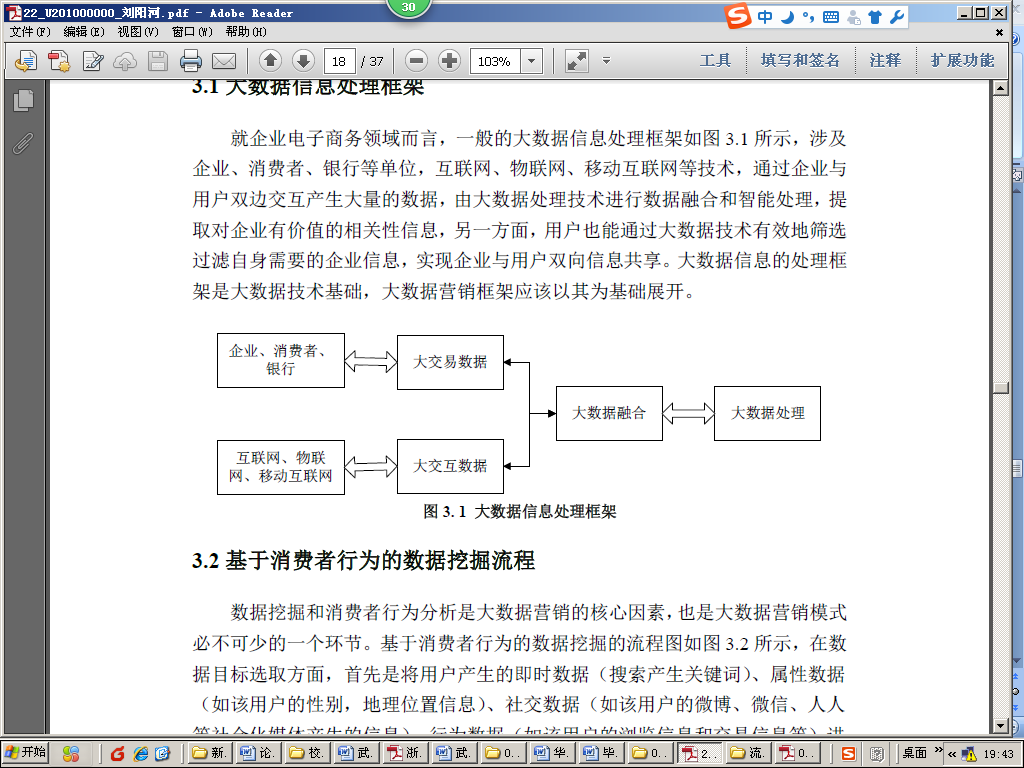
\includegraphics[width=0.5\textwidth]{fig/testmindmap}
	\caption{测试图片, 因为学校模板给的word中的图片就是从这上面截取的部分,所以另存为PNG之后就是这个样子}
	\label{testfig}
\end{figure}
$ \times\times\times\times\times\times\times\times\times\times\times\times\times\times\times\times\times\times\times\times $  (如\reffig{E8} 所示)
\begin{figure}[H]
	\centering
	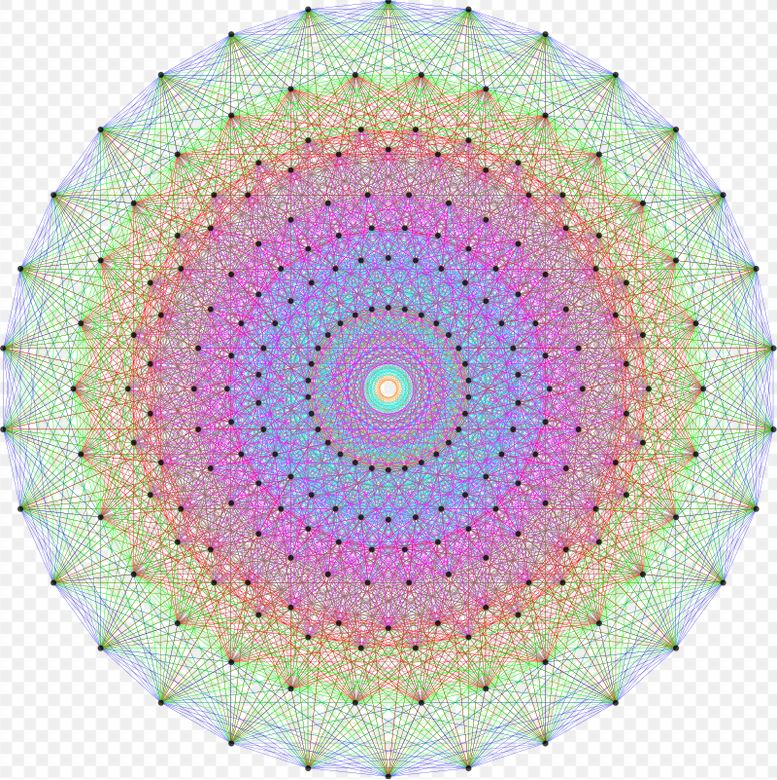
\includegraphics[width=0.5\textwidth]{fig/E8Petrie}
	\caption{测试图片: E8 李群}
	\label{E8}
\end{figure}
\textcolor{red}{(图标题:位于图下方,黑体小4号,字母、阿拉伯数字为Time New Roman 小4号)}

\sectionbreak
% 参考文献 %
\clearpage
\phantomsection
\addcontentsline{toc}{section}{参考文献}
\bibliographystyle{plain}
\bibliography{cite}\label{bibtexref}
%  附录  %
\clearpage
\appendix
\phantomsection
\addcontentsline{toc}{section}{附录(源码展示)}
\section*{附录(源码展示)}
% 重置附录 section 格式
\renewcommand{\thesubsection}{\thesection\Alph{subsection}}
\subsection{前端代码结构}
\subsection{后端代码结构}

\end{document}